\chapter{Models of Computation}
\label{cha:models}


A \emph{model of computation} describes what computation is and how it
is done. The best known is Alan Turing's model~\cite{Turing} in which
a machine manipulates the contents of a tape according to a finite set
of instructions. It has become the yardstick with which we measure
other models of computation. Turing's notion of computability is very
robust. First it is robust because changes to the definition of Turing
machines, such as increasing the number of tapes or heads, or allowing
the head to jump around, does not change the computational
power.\footnote{We are ignoring questions of computational
  \emph{complexity}.} The notion is also robust because many other
definitions of computation turned out to be equivalent to Turing's in
the sense that machines of one kind can simulate those of the other
kind, and vice versa.

However, we would commit a serious mistake if we concluded that by
studying only Turing machines we will learn everything there is to
learn about computable mathematics. Our inquiry into the nature of
computation, especially computation with infinite structures, will
reveal a plethora of possibilities which are \emph{not} equivalent.
Thus we begin the chapter with a review of several models of
computation. We then discuss the question of what a model of
computation might be in general, and how such models are compared.


\section{Turing machines}
\label{sec:turing-machines}

We recall informally how a Turing machine operates. There is little
point in giving a formal definition because we do not intend to
actually write programs for Turing machines. If you are not familiar
with Turing machines, see the section on further reading at the end of
the chapter.

\begin{figure}[htbp]
  \centering
  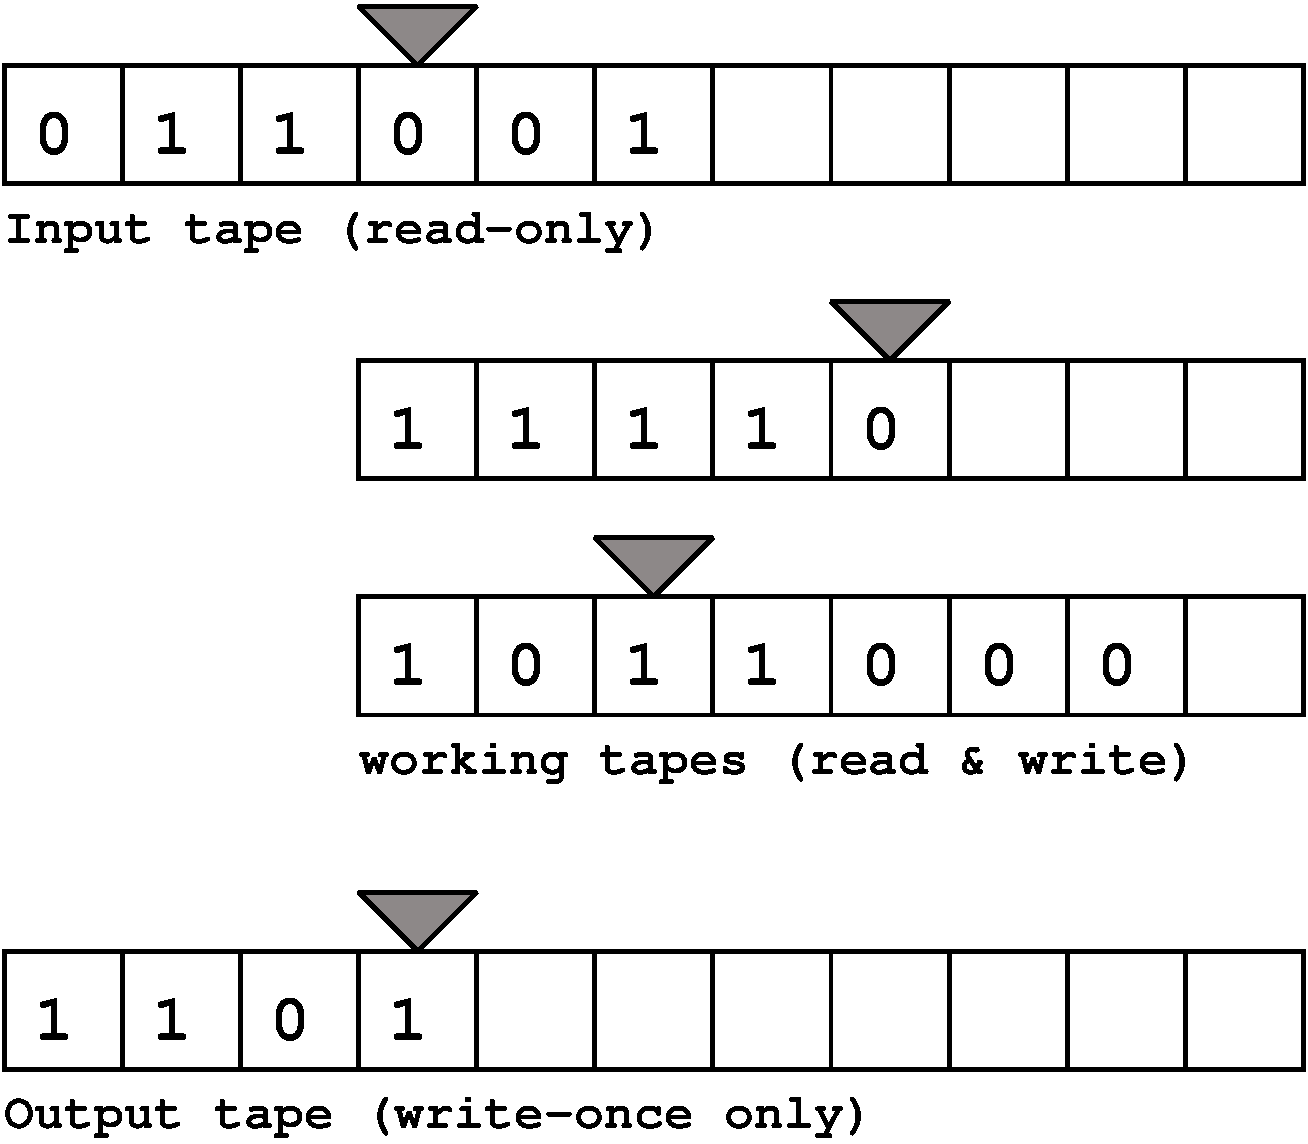
\includegraphics[width=0.5\textwidth]{turing_machine}
  \caption{A Turing machine operates with tapes}
  \label{fig:turing-machine}
\end{figure}

A Turing machine is a device which operates on a number of tapes and
heads, see Figure~\ref{fig:turing-machine}:
%
\begin{itemize}
\item the input tape is equipped with a reading head which can move
  left and right, and read the symbols but cannot write them.
\item The working tapes are equipped with heads that move left and
  right, and can both read and write symbols.
\item The output tape is equipped with a write-once head which starts
  at the left-most end. Each time the head writes a symbol it
  automatically moves to the right by one place. It cannot move to the
  left, and only moves to the right after writing a symbol.
\end{itemize}
%
The tapes are infinite\footnote{If you are worried about having actual
  infinite tapes in your room, note that at each step of the
  computation only a finite portion of tapes has been inspected. In
  this sense the tapes are \emph{potentially} infinite.} and contain
symbols from a given finite alphabet. A common choice for the alphabet
is $0$, $1$, and a special symbol `blank'. The machine manipulates the
contents of the tapes according to a \emph{program}, which is a finite
list of simple instructions that manipulate the heads and the tapes.
The machine executes one instruction at a time in a sequential manner.
It may \emph{terminate} after having executed finitely many
computation steps. If it does not terminate then it runs forever, in
which case we say that it \emph{diverges}.

Our version of Turing machine is different from the usual one, where a
machine is equipped with only a single tape that serves for input,
output, and intermediate work. The two formulations are equivalent in
the sense that a single-tape machine can simulate the workings of a
Turing maechine with several tapes, and vice versa. Our formulation
will ease the description of infinite computations in
Section~\ref{sec:type-2}.

The state of a Turing machine may be encoded onto a single tape as
follows. First we write down the program, suitably encoded by the
symbols from the alphabet, then the current state (the next
instruction to be executed), and positions of the heads. Finally, we
copy the contents of all the tapes by interleaving them into a single
tape.

If we were going to build just one machine, which one would we build?
The answer was given by Turing.

\begin{theorem}[Turing]
  There exists a \emph{universal} machine---a machine that takes a
  description of another machine, as explained above, and simulates
  it.
\end{theorem}

\begin{proof}
  A traditional proof may be found in any book on computability
  theory, and there is nothing wrong with reading the original
  proof~\cite{Turing} either. A different kind of a proof is the
  observation that you use universal machines every day.\footnote{You
    have to ignore the fact the several hundred gigabytes of storage
    are not quite the same thing as an infinite tape. Also, modern
    compuers are really universal \emph{Von Neumann}
    machines~\cite{vonNeumann} because they have a central processing
    unit and random access memory instead of a tape.}
\end{proof}

Once we have a universal machine, we can make it behave like any other
machine. It is just
\href{http://www.catb.org/jargon/html/S/SMOP.html}{``a simple matter
  of programming''} to tell it what to do.

We mentioned in the introduction that many kinds of computing devices
are equivalent to Turing machines. We shall therefore not insist on
describing computation solely in terms of Turing machines, but rather
rely on familiarity with modern computers and programming languages.
After all, programs can actually be run on computers, whereas Turing
machines are rather hard to get by.

\subsection{Type 1 machines}
\label{sec:type-1}

Enumeration of Turing machines.

Partial computable functions.

Halting oracle.

s-m-n

u-t-m

\subsection{Type 2 machines}
\label{sec:type-2}

\subsection{Sequential machines}
\label{sec:sequential-machines}


\section{The graph model}
\label{sec:graph-model}


\section{Partial combinatory algebras}
\label{sec:pcas}

\subsection{$\lambda$-calculus}
\label{sec:lambda-calculus}




\section{Real-world programming languages}
\label{sec:programming-languages}


\section{Comparison of models of computation}
\label{sec:models-comparison}



\section{Further reading}
\label{sec:models-further-reading}

As a general introduction to Turing machines and classical
computability theory I recommend Piergiorgio Oddifreddi's
book~\cite{Oddifreddi}. Also suitable and perhaps more readily
available textbook is Hartley Rogers~\cite{Rogers}. If you would like
to see Turing machines done rigorously and in gory detail, look at
Martin Davis's booklet~\cite{Davis}.



%%% Local Variables: 
%%% mode: latex
%%% TeX-master: "notes"
%%% End: 
